% Autor: Dominik Harmim <harmim6@gmail.com>

\documentclass[a4paper, 10pt, twocolumn]{article}

\usepackage[czech]{babel}
\usepackage[utf8]{inputenc}
\usepackage[T1]{fontenc}
% \usepackage[left=2cm, top=2cm, text={17cm, 25cm}]{geometry}
\usepackage[left=2cm, top=1.6cm, text={17cm, 25.5cm}]{geometry}
\usepackage[unicode, colorlinks, hypertexnames=false, citecolor=red]{hyperref}
\usepackage{times}
\usepackage{graphicx}


\begin{document}
    \twocolumn[
        \begin{@twocolumnfalse}
            \begin{center}
                {\Large
                    Vysoké učení technické v~Brně \\
                    Fakulta informačních technologií \\
                }
                {
\includegraphics[width=.4 \linewidth]{img/FIT_logo.pdf}} \\

                {\LARGE
                    Paralelní a~distribuované algoritmy \\
                    3.~Projekt\,--\,Viditelnost \\[.4cm]
                }

                {\large
                    Dominik Harmim (xharmi00) \\
                    \texttt{xharmi00@stud.fit.vutbr.cz} \\
                    \today
                }
            \end{center}
        \end{@twocolumnfalse}
    ]


    \section{Rozbor algoritmu}

    Implementovaný algoritmus řeší problém tzv. \emph{viditelnosti},
    anglicky zvaný \emph{Line-of-Sight}. Tento problém je definován
    následovně. Je dána dvou-rozměrná matice terénu ve formě nadmořských
    výšek a~pozorovací bod (\emph{místo pozorovatele}). Je třeba zjistit,
    které body podél paprsku vycházejícího z~místa pozorovatele určitým
    směrem jsou viditelné. V~rámci tohoto projektu je problém zjednodušen
    tím způsobem, že je dána pouze \emph{sekvence bodů}, která reprezentuje
    nadmořské výšky terénu podél pozorovacího paprsku. První bod v~této
    sekvenci je nadmořská výška místa pozorovatele.

    Algoritmus, který řeší tento problém, označí body podél pozorovacího
    paprsku jako viditelné, pokud žádný bod mezi pozorovatelem a~těmito
    body nemá větší \emph{vertikální úhel}. Nejdříve se vektor výšek
    bodů podél pozorovacího paprsku přepočítá na vektor vertikálních
    úhlů. Následně se spočítá \emph{vektor maximálních úhlů} pomocí
    operace \emph{prescan} s~operátorem \emph{maximum}. Pro zjištění
    viditelnosti bodu stačí porovnat jeho vertikální úhel s~patřičným
    maximem.

    \subsection{Analýza algoritmu}

    Algoritmus provádí operaci \emph{prescan}, která předpokládá takový
    počet procesů, který je \emph{mocninou čísla~2}. Zároveň každý proces
    pracuje se dvěma body. Počet prvků je vždy zaokrouhlen na
    \emph{nejbližší vyšší} mocninu čísla~2. V~nejlepším případě, kdy počet
    bodů~$ n $~podél pozorovacího paprsku je mocninou čísla~2, je
    \emph{počet procesů pro výpočet} $ p(n) = \frac{n}{2} $. V~nejhorším
    případě je $ p(n) = n - 1 $.

    \emph{Prostorová složitost} je $ s(n) = p(n) \cdot 2 $, protože každý
    proces pracuje se dvěma body. Pokud je počet bodů mocninou čísla~2,
    potom je $ s(n) = n $ a~všechen prostor je maximálně využit. V~opačném
    případě je ale určitý prostor vyplněn \emph{neutrálními prvky}.

    V~algoritmu každý proces paralelně provádí výpočet vertikálních úhlů
    svých bodů a~porovnání vypočítaných úhlů s~patřičnými maximálními úhly.
    Toto se provede v~\emph{konstantním čase}. Výpočet maximálních úhlů
    se provádí operací \emph{prescan}, která má \emph{logaritmickou} časovou
    složitost. \emph{Celková časová složitost} je tedy $ t(n) =
    \mathcal{O}(\log p(n)) $.

    \emph{Celková cena} tohoto algoritmu je následující: $ c(n) = t(n)
    \cdot p(n) = \mathcal{O}(\log p(n)) \cdot p(n) = \mathcal{O}(\log(p(n))
    \cdot p(n)) $. Tato cena \emph{není optimální}, protože $ \mathcal{O}(
    \log(p(n)) \cdot p(n)) \neq \mathcal{O}(n) $, kde $ \mathcal{O}(n) $ je
    cena \emph{optimálního sekvenčního řešení} tohoto algoritmu. Algoritmus
    by byl optimální, pokud by se snížil počet procesů a~každý proces by
    zpracovával několik bodů sekvenčně a~pokud by platilo, že $ \log p(n)
    < \frac{n}{p(n)} $.

    \emph{Zrychlení} tohoto algoritmu oproti optimálnímu sekvenčnímu řešení,
    které má časovou složitost $ t(n) = \mathcal{O}(n) $, je následující:
    $ \frac{\mathcal{O}(n)}{\mathcal{O}(\log p(n))} $.


    \section{Implementace}

    Algoritmus je implementován v~programovacím jazyce C++. Je využito
    knihovny \emph{Open MPI} pro zasílání zpráv mezi procesy. Implementace
    se nachází v~souboru \texttt{vid.cpp}. Po spuštění programu se hned
    po inicializaci knihovny Open MPI zjistí číslo procesu, která mu
    knihovna přidělila. Podle tohoto čísla se potom rozhoduje, jak se
    bude daný proces chovat a~se kterými procesy bude komunikovat. Procesy
    se číslují přirozenými čísly včetně čísla~0. Proces s~číslem~0, tzv.
    \emph{hlavní proces}, je proces, který provádí vstupní a~výstupní
    operace a~který iniciuje komunikaci s~ostatními procesy a~celou
    komunikaci řídí. Program je rozdělen do několika částí, které budou
    popsány v~následujících odstavcích.

    Před samotným spuštěním programu je nejdříve potřeba říct, kolik
    procesů bude pro výpočet potřeba. Při spouštění programu připraveným
    skriptem \texttt{test.sh} je tento počet automaticky spočítán. Skript
    nejdříve zkontroluje validitu vstupní sekvence bodů. Pokud
    je tato validní, vypočítá se potřebný počet procesů následujícím
    výrazem $ \frac{2^{ceil(\frac{\log n}{\log 2})}}{2} $, kde~$ n $~je
    počet bodů podél pozorovacího paprsku a~$ ceil $ je funkce, která
    zaokrouhlí dané číslo na nejbližší vyšší celé číslo. Jinými slovy,
    počet procesů je polovina počtu bodů podél pozorovacího paprsku
    zaokrouhlená na \emph{nejbližší vyšší} mocninu čísla~2.

    V~první části programu hlavní proces provádí funkci
    \texttt{send\_alts}, kde se znovu provede validace vstupní sekvence
    bodů a~kontrola, zda byl program spuštěn se správným
    počet procesů (pro případ, že by program nebyl spuštěn připraveným
    skriptem). Následně se provede rozeslání vstupních bodů všem
    procesům. Každý z~procesů obdrží dva po sobě jdoucí body a~bod místa
    pozorovatele. Protože počet procesů byl zaokrouhlen na nejbližší
    vyšší mocninu čísla~2, sekvence vstupních bodů je doplněna speciálními
    prázdnými hodnotami tak, aby každý proces obdržel dva body. Všechny
    procesy následně provádí funkci \texttt{receive\_alts}, která přijímá
    patřičné vstupní body od hlavního procesu.

    V~další části programu nejdříve všechny procesy paralelně volají funkci
    \texttt{calculate\_angles}, která počítá \emph{vertikální úhly} daných
    bodů od místa pozorovatele. Dále se volá funkce \texttt{max\_prescan},
    která provádí operaci \emph{prescan} s~binárním asociativním operátorem
    \emph{maximum} a~s~\emph{neutrálním prvkem}, který je roven nejmenší
    možné hodnotě úhlu (konkrétně v~C++ je to
    \texttt{numeric\_limits<double>::lowest}). Jedná se o~částečný výpočet
    \emph{sumy prefixů}. Provádí se zde operace \emph{up-sweep},
    která vypočítá maximální úhel a~zároveň jsou ukládány mezivýsledky.
    Nejdříve je paralelně vypočítáno maximum každých dvou úhlů, dále
    každých čtyřech úhlů atd. Výpočet končí po $ \log_2 n $ krocích,
    kde~$ n $~je počet úhlů. Následně se provádí operace \emph{down-sweep},
    která nejprve do posledního úhlu uloží neutrální prvek a~dále se
    paralelně zpracovávají každé $ \log_2 n $ úhly, následně každé
    $ \log_2(n) - 1 $ úhly atd. Výpočet končí po $ \log_2 n $ krocích.
    V~každé úrovni zpracování pošle proces svůj úhel procesu vlevo od
    něj, se kterým komunikuje a~dále vypočítá maximum z~původního levého
    úhlu a~ze svého úhlu.

    Konečně se paralelně vypočítají viditelnosti bodů podél pozorovacího
    paprsku porovnáním svých úhlů s~patřičným vypočítaným maximum
    a~výsledná viditelnost se pošle hlavnímu procesu. Toto se provádí
    ve funkci \texttt{send\_visibility}. Hlavní proces potom už jen volá
    funkci \texttt{receive\_visibility}, která přijímá vypočítané
    viditelnosti všech bodů a~potom volá funkci \texttt{print\_visibility},
    která tyto výsledné viditelnosti vypisuje na standardní výstup.

    Na obrázku~\ref{fig:seq-diagram} je sekvenční diagram, který znázorňuje
    výše popsanou komunikaci mezi procesy.

    \begin{figure}[ht]
        \centering
        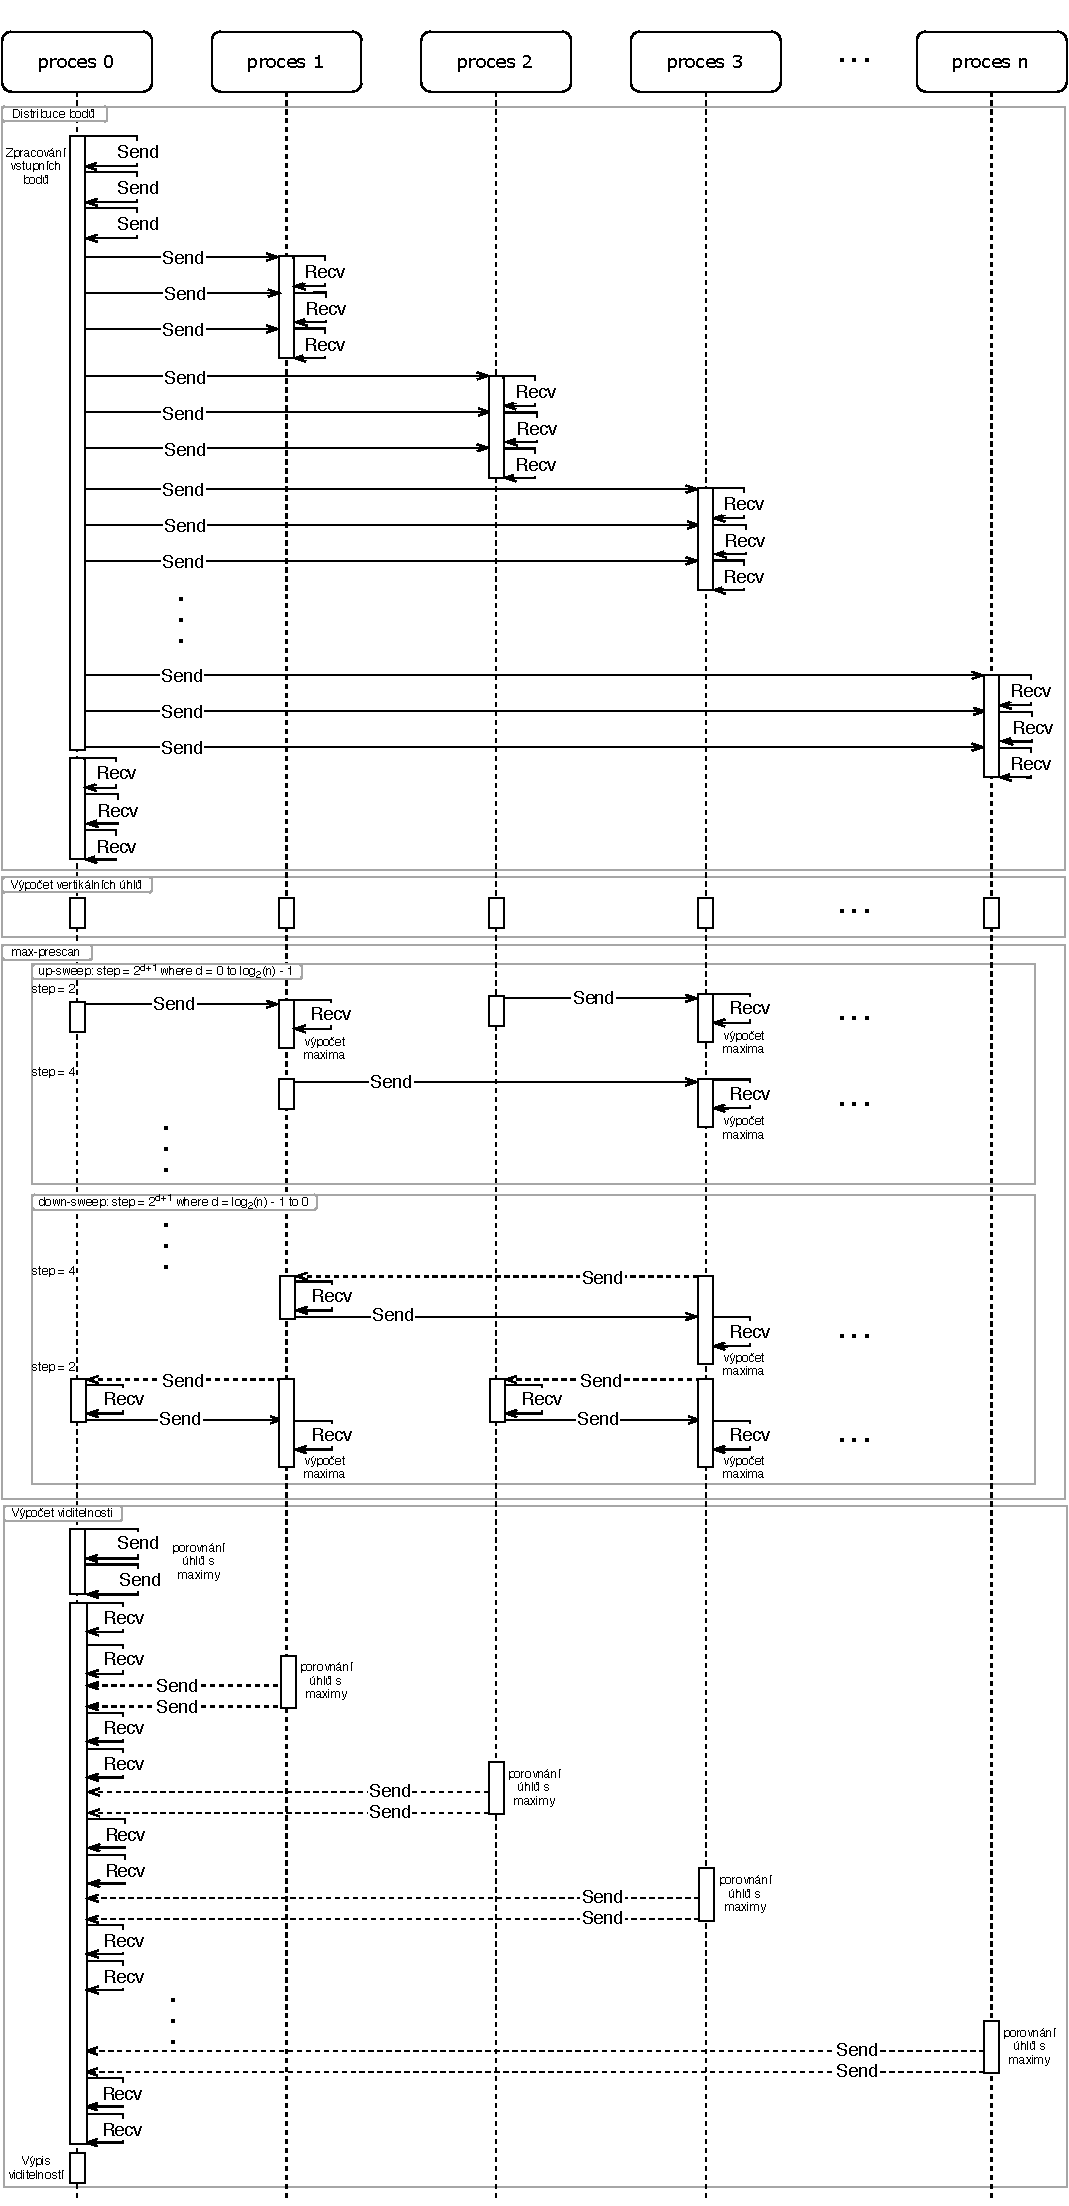
\includegraphics[width=.95 \linewidth]{img/sequence-diagram.pdf}
        \caption{Komunikační protokol procesů}
        \label{fig:seq-diagram}
    \end{figure}


    \section{Experimenty}

    Pro ověření \emph{teoretické časové složitosti} byly provedeny
    experimenty, kde byl měřen \emph{reálný čas} provádění algoritmu funkcí
    \texttt{std::chrono::high\_resolution\_clock::now}. Měření bylo
    prováděno na superpočítači Salomon pro různý počet bodů od~4 až
    do~32 bodů. Každé měření pro určitý počet bodů bylo prováděno několikrát
    a~výsledky byly průměrovány, aby nebyly vidět případné odchylky.
    Výsledky tohoto měření jsou k~vidění na obrázku~\ref{fig:experiment}.
    Je zřejmé, že reálná časová složitost roste přibližně
    \emph{logaritmicky}, stejně jako teoretická.

    \begin{figure}[ht]
        \centering
        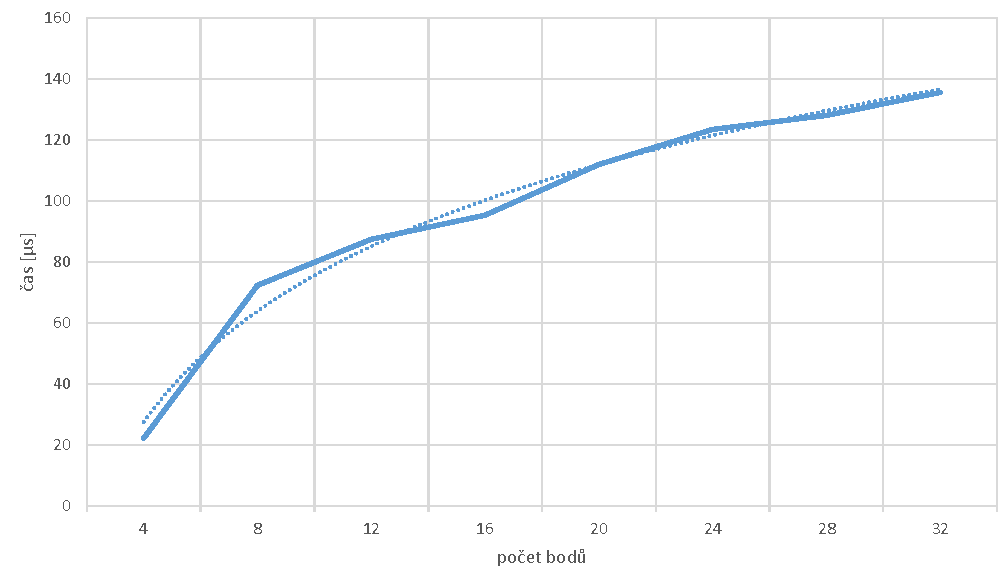
\includegraphics[width=1 \linewidth]{img/experiments.pdf}
        \caption{Výsledky měření experimentů}
        \label{fig:experiment}
    \end{figure}


    \section{Závěr}

    V~rámci tohoto projektu byla úspěšně vytvořena implementace algoritmu,
    který řeší problém \emph{viditelnosti}. Teoretická časová složitost
    tohoto algoritmu byla ověřena reálnými experimenty.
\end{document}
